\chapter{RTOS outline}

In this chapter, we will cover the specificities of each OS we planned to work with.
We chose to write about technical and non-technical characteristics of the chosen OS and even their respective projects as a whole.

%Some of the things written in this chapter are personal opinions.
%Indeed, as we decided to include non-technical characteristics of each of the projects, some subjectivity is involved.
%We tried to be critical and impartial in those points but it beware it only reflects our own opinions.

A table summarizing the comparison is provided at the end of the chapter.

%https://www.simform.com/iot-rtos-selection/
%https://ijarcce.com/wp-content/uploads/2015/12/IJARCCE-92.pdf
%http://www.ipcsit.com/vol1/54-S028.pdf

%Supported Architecture
%License
%User-friendly/documentation/example applications
%Supported network protocols
%kernel type
%date of creation
%file systems supported
%number of boards supported
%memory footprint
%resource access control (posix...)
%memory management policy
%energy management features
%programming model
%scheduling
%community
%build system
%ipc management

\section{RIOT}
%TODO explain why we chose riot

\subsection{Historic}

The RIOT project started privately in 2008.
It started as a part of the FeuerWhere project (\url{http://feuerwhere.mi.fu-berlin.de}), 
    where firefighters would be tracked with embedded devices during an intervention.
The goal was to design an ad hoc self-configurating network of sensors used 
    to monitor vital state and environmental parameters of rescue forces inside a building.

% https://ieeexplore.ieee.org/stamp/stamp.jsp?tp=&arnumber=6142316
In 2010, a fork from the FeuerWare software developed for the FeuerWhere project was made.
Development continued for $\mu$kleos\cite{microkleos}, a microkernel-based operating system for embedded devices.
The focus of this system was modularity and Internet compliance with the integration of IETF protocols such as 6LoWPAN, RPL and TCP.

In 2013, RIOT went public.
$\mu$kleos was rebranded to avoid problems with spelling and pronunciation.
Since then, more than 200 people contributed to the project with more than 20 000 commits and 75 releases.
The project is currently supported by Freie Universität Berlin, INRIA and Hamburg University of Applied Sciences.

\subsection{Characteristics and features}
%ce que fait l'os
%https://www.osrtos.com/rtos/riot/
RIOT is an open-source real-time operating system.
The OS provides a lightweight operating system with multithreading and real-time features running across a wide range of resources constrained devices.
It runs on 8-bit, 16-bit and 32-bit platforms and only needs a minimum of 1,5 kB of RAM.
A focus has been made on making RIOT standard-C and C++ compliant.

\paragraph{License} RIOT is distributed under the LGPL2.1 license which provides unrestricted commercial or private use, modification and distribution if it is not a derivative work.
With LGPL license, RIOT is also provided "as is", without any warranty of any kind.

\paragraph{Technicals} The RIOT project aims to bridge the gap between operating systems for Wireless Sensor Networks (WSN) and traditional fully fledge operating systems.
RIOT follows some design objectives such as:
\begin{itemize}
    \item Energy efficiency
    \item Small memory footprint
    \item Modularity
    \item Uniform API, platform agnostic
\end{itemize}

%https://github.com/RIOT-OS/RIOT/wiki/RIOT-Community-Processes
\paragraph{Community} The RIOT community can be characterized in 3 categories\cite{RIOTComm}:
\begin{itemize}
    \item Contributors are people who contributed to the project, from code contribution to technical or non-technical discussions.
    \item Maintainers who contributed noticeably on the project.
        Maintainers can propose to give the maintainer status to contributors that have been noticed.
        The status comes with rights (merge rights) and duties (code review duties).
    \item Coordinator status is acquired following the same principle as the maintainer.
        The role covers non-technical aspects of the project such as bringing up topics, debates and deal with the overhead.
\end{itemize}

\subsection{Specificities}
%https://hal.inria.fr/hal-00768685v1/document
%static memory for the kernel
%dynamic memory
RIOT enforces constant time for kernel tasks.
The kernel exclusively uses static memory which guarantees runtimes of \textit{O}(1) whereas dynamic memory is used for applications.

The scheduler cycle is also performed in constant runtime thanks to a circular linked list of threads\cite{riotspec}.

%tickless
The main specificity of RIOT resides in its scheduler.
The operating system includes a tickless scheduler.
When there is no pending task, the operating system will switch to the \textit{idle} task which is the thread with the lowest priority.
The CPU will then put itself in its deepest possible sleep mode (which depends on the device in use).
In this state, the device can only be woken up by an interrupt (external or kernel-generated).
\section{Contiki}
%https://komalbattula.wordpress.com/architecture/
%explain contiki and why we chose it

\subsection{Historic}
%https://ieeexplore.ieee.org/stamp/stamp.jsp?tp=&arnumber=1367266
%https://ercim-news.ercim.eu/en76/rd/contiki-bringing-ip-to-sensor-networks
Contiki was created in 2003 by Adam Dunkels. %http://dunkels.com/adam/
At the time, it was the first operating system to provide IP connectivity to sensor networks.
It did so thanks to $\mu$IP, a lightweight TCP/IP stack intended for tiny microcontrollers,
    also developped by Adam Dunkels at the Swedish Institute of Computer Science (now RISE SICS).%https://github.com/adamdunkels/uip

Further developpement of Contiki has been supported by various industries and research institutes 
    such as Texas Instruments, Atmel, Cisco, ENEA, ETH Zurich, Redwire, RWTH Aachen University, 
    Oxford University, SAP, Sensinode, Swedish Institute of Computer Science, ST Microelectronics and Zolertia.
%death?

\subsection{Characteristics and features}
The developpement of Contiki started with the need to bring connectivity to small sensor devices with limited capabilities.
By definition, Contiki is not a real-time operating system and has not been designed as such.\\

%memory allocation/stack and kernel/event driven
Contiki operates with the event-driven model.
Processes are implemented as event handlers that run to completion.
An event handler can be defined as a procedure that performs a specific action in response to an event.
Because event handlers cannot block, the same stack can be shared among them.
Also, locking mechanisms are not needed as event handlers do not run concurrently.
Instead of having multiple stacks for multiple threads (which must be over-provisioned or they risk to run out of memory), a single stack can then be used.

This model does not come without problems, as it is sometimes tedious for programmers to manage.
For example, a time-consumming process such as a cryptocraphic operation can monopolize the CPU for quite some time 
    and make the system unable to respond to external events. 
In a preemptive multi-threading system, the computation can be preempted to react to an external event 
    and continue the process later.
To fix this issue, Contiki makes use of an application library that implements preemptible threads.
This library is optional an can be used with programs that explicitly require it.\\

%protothreads
%http://dunkels.com/adam/dunkels05using.pdf
In order to implement its event-driven system, Contiki comes with a mechanism called \textit{protothread}.
The concept of protothreads was also developped by Adam Dunkels with the help of other researchers.
The goal of the protothread programming abstraction is to make it easier for developpers to develop, debug and maintain code written in the event-driven model.

Protothreads can be defined as lightweight stackless threads providing a blocking context on top of an event-driven system.
They can be used to perform non-preemptive concurrency or cooperative multitasking.
Programs written for an event-driven model typically have to be implemented as explicit state machines.
With protothreads, programs can be written in a sequential fashion without designing explicit state machines.

Protothreads do not serve the same purpose as threads for the event-driven model.
The concept has been developped to bring a number of benefits of the multi-threaded programming model into Contiki
    and ease the developpement of applications.\\

%energy saving mechanisms
Contiki does not provide any specific kernel energy saving mechanism.
Instead, it let the application specific parts of the system implement such mechanism.

\subsection{Specificities}
%contiki is specific by itself, aims for WSN
%dynamic loading? is that necessary to develop that?
%cooja
Contiki integrates a tool called Cooja.
Cooja is a network simulator which is designed to simulate a network using Contiki motes.
Motes can be simulated at the hardware level or with a standard setup allowing faster response but with less precise system behaviour.
It is an extremely powerful tool which makes developping and debugging tremendously easier even with a large-scale network.

\begin{figure}[!h]
    \centering
    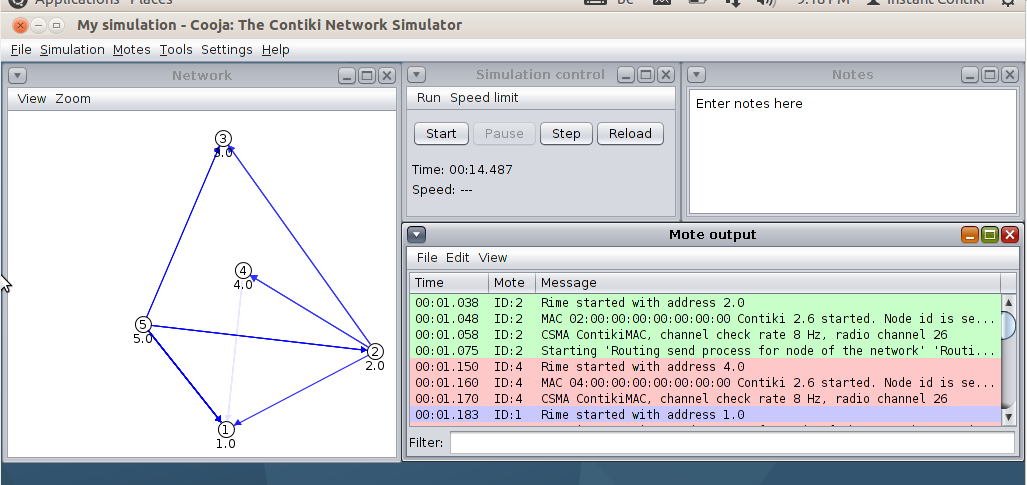
\includegraphics[scale=0.4]{assets/cooja.png}
    \caption{\label{fig:cooja}Cooja interface}
\end{figure}

%rime https://pdfs.semanticscholar.org/9feb/7e0f0d3b507f2f3da60c1b2fea9d5e43449d.pdf
%Contiki provides a low-power radio networking stack called Rime.
%This stack can be used where the full IP stack is not needed.
%The Rime stack can be tuned to 
\section{FreeRTOS}

\subsection{Historic}
\paragraph{}
%https://www.freertos.org/RTOS.html
The FreeRTOS kernel has been developped in 2003 by \href{https://www.linkedin.com/in/richard-barry-4562262/}{Richard Barry}. %fix href pls
He founded a company called Real Time Engineers Ltd to develop and maintain FreeRTOS until the stewardship of the project was passed to Amazon Web Services in 2017.
Since then, we can distinguish the FreeRTOS kernel and Amazon FreeRTOS which includes the aforementioned kernel 
    with a set of libraries extending the functionalities of the RTOS.

\subsection{Characteristics and features}
\paragraph{}
%real time
Similarly to RIOT OS, FreeRTOS is designed to be a real-time preemptive operating system aimed at embedded devices.
Its strength comes from the fact that it is highly and easily configurable.\\

%scheduler
%http://richardgoyette.com/Research/Papers/FreeRTOSPaper.pdf
For example, FreeRTOS supports preemptive or cooperative scheduling. 
It also uses Dynamic Priority Scheduling which means that the priorities are defined during runtime.
The user can choose which scheduling policy he wants by modifying the \texttt{configUSE\_PREEMPTION} variable in the \texttt{FreeRTOSConfig.h} file.
In the cooperative case, the only action the scheduler performs is to increase the tick count.
In the preemptive case, the scheduler increments the tick count and then checks if a task is in the unblocked state.
If it is indeed the case, it checks the priority level of the task and compares it with the current task to see if a switch is required.\\

%tasks and coroutines
%https://www.freertos.org/taskandcr.html
%https://www.researchgate.net/profile/Ming_Yuan_Zhu/publication/308692183_Understanding_FreeRTOS_A_Requirement_Analysis/links/57eb301108ae5d93a4816184.pdf
Since FreeRTOS uses the multi-threading paradigm, the code can be structured as a set of tasks.
As explained in the first chapter, each task use its own stack and therefore has its own context.

In addition to tasks, FreeRTOS includes a another mechanism called \texttt{co-routine}.
Co-routines are similar to tasks but have some fundamental differences which justify their usage:
\begin{itemize}
    \item They share the same stack between them which greatly decrease the memory wasted in provisioning.
    \item They use a cooperative scheduling between them but they can be used in an application using preemptive tasks.
    \item The shared stack comes with more restrictions on how co-routines can be structured compared to regular tasks.
\end{itemize}
Co-routine have been implemented for very RAM constrained devices and are very rarely used those days.
Nonetheless, they stay a relevant alternative to tasks for specific usages.\\
%ipc
%deadlock avoidance
%scheduler suspension
FreeRTOS also supports tickless idle mode, similarly to RIOT.
Since FreeRTOS is highly configurable, the developer can activate this feature 
    by setting the variable \texttt{configUSE\_TICKLESS\_IDLE} as 1 in \texttt{FreeRTOSConfig.h}.
A custom built tickless idle mode can also be provided by the developer and used by setting the same variable to 2.
This feature can be used when a default implementation in not provided for a certain board.
%memory allocation
\section{Comparison Table}